\subsection{Project characteristics}
% Charakterystyka projektu i sposób jego realizacji - macie tutaj napisać co to był za projekt (badawczy, rozwojowy) a wiec czy wymagania były jasne czy tak naprawdę powstawały w jego trakcie. Ważne by spróbować scharakteryzować przyjęty sposób realizacji a wiec przyjęty proces np. czy to był proces przyrostowy czy iteracyjny. Najczęściej Wasz proces jest oparty na prototypowaniu z odrzucaniem przez pierwszy semestr, a potem to typowy proces przyrostowo-iteracyjny w drugim semestrze. Spróbujcie napisać również z czego to wynika.

Our projects is special for a few reasons.

First of all, we came up with a project idea ourselves and tried to find a person that would be interested in being a thesis supervisor.
Taking that into account, the requirements for the project were not defined beforehand
and we learned more and more about them as the project developed.
Due to that fact, it was both easier and harder for us to do our job as architects and developers.
On the one hand, it was mostly us who were responsible for the direction the project would take, but at the same time, at each step of the process
we had to struggle with choosing which parts of the project would be more attractive for our client, our future users, and from the scientific point of view.

Second of all, some of the problems we were faced with come from the field of \textit{Computational Origami}.
It's a relatively new branch of science, which ideas span the realms of mathematics, physics, 
computer science, engineering, and even architecture.
Also, it is not a subject that would normally be taught during one's educational career.
Of much help to us was Prof. Erik Demaine and his MIT course on Geometric Folding Algorithms: Linkages, Origami, Polyhedra \cite{mit-course}
\smallskip

Taking into consideration all the facts mentioned above, our work did not have a specifically structured approach.
We were working in a very simplified \textbf{Kanban} method, where we would select things to work on
as the project unfolded. 
\smallskip

For the better part of the first semester,
we were creating a prototype that would serve as a \textit{Minimal Valuable Product}.
Later on, we did not discard it altogether, but started adding more features on top of it,
polishing it and refactoring when necessary. 
We continued with this approach till the end.

\subsection{Team}
% Osoby w projekcie - często projekt jest robiony dla kogoś a opiekun ma jakieś osoby pomocnicze. Wskażcie wszystkie osoby i ich role w projekcie. Bardzo ważny punkt z formalnego widzenia projektu, gdyż każda osoba musi zostać oceniona w sposób indywidualny.

Our team consisted of our thesis supervisor and us.

\begin{enumerate}
	\item \textbf{Witold Alda} - thesis supervisor.
	\item \textbf{Maciej Mionskowski} - developer, architect.
	\item \textbf{Antoni Mleczko} - developer, architect.
\end{enumerate}

\subsection{Responsibilities in the team}
% Zespól i podział obowiązków - musicie napisać co kto robił. Jeśli wszystko robiliście razem to spróbujcie wskazać chociaż 2-3 główne zadania, którymi każde z Was się zajmowało.

Although we were distributing workload equally between the team members
and each of us touched on all parts of the project, some areas 
received more attention from one person than the other.
To be able to define how much of a percentage each one of us has contributed to the 
given area of the project, first we need to define those areas.
\smallskip

Project areas:
\begin{itemize}
	\item Solver backend
	\item Frontend
	\item Community backend
	\item DevOps / Infrastructure
	\item Thesis
	\item Research
	\item Requirements formulation
\end{itemize}

Having defined project areas, we have agreed upon how much of a contribution each of
us has provided to the given area.

\begin{figure}[H]
  \caption{Maciej's percentage contribution to the areas of the project.}
  \centering
  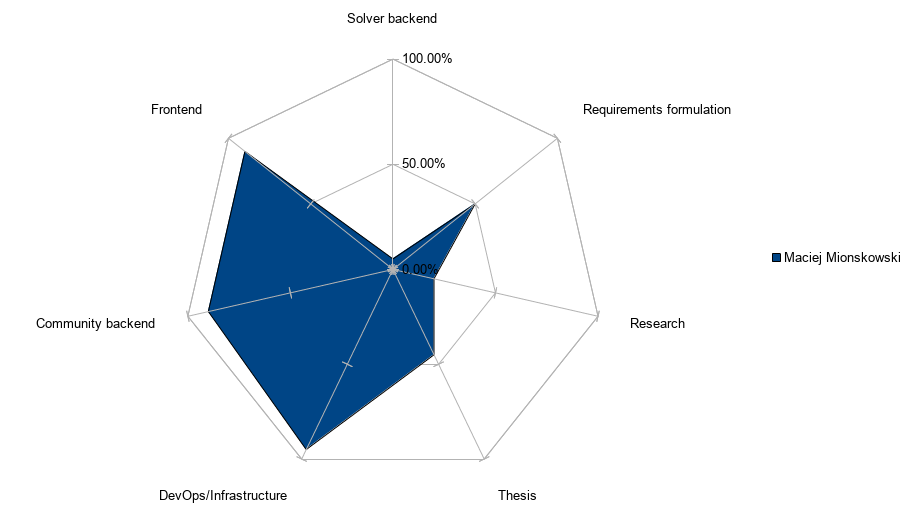
\includegraphics[width=\textwidth]{assets/4-percentage-maciej.png}
\end{figure}

\begin{figure}[H]
  \caption{Antoni's percentage contribution to the areas of the project.}
  \centering
  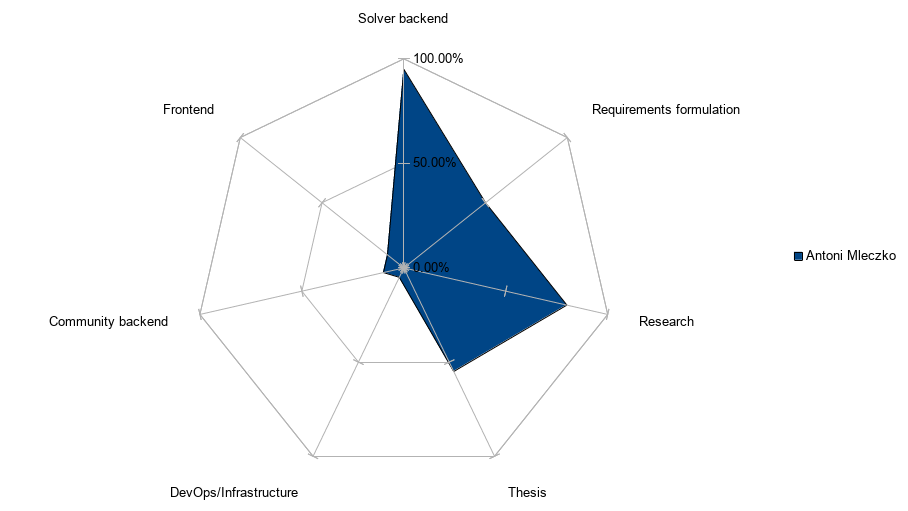
\includegraphics[width=\textwidth]{assets/4-percentage-antoni.png}
\end{figure}




\subsection{Organization of work}
% Organizacja prac i wykorzystane narzędzia - używaliście facebooka, emaili czy spotykaliście się zawsze o określonej porze? Jak i kiedy dzieliliście się zadaniami: czy było to po każdym spotkaniu z klientem? Kiedy spotykaliście się z klientem? Jak często? Używaliście Jiry, confluence, trello? Koniecznie zróbcie screenshota! A może jakieś statystyki z githuba które jakoś podsumują Wasz projekt? Tutaj Wasze przemyślenia i komentarze mile widziane.
% Zastosowane techniki i praktyki - odnosi się do powyższego, ale możecie tutaj spróbować wskazać takie praktyki jak Pair Programming, TDD, Refactoring, Planning Game, User Stories, Team Velocity, Continuous Integration, Sprint Review Meeting, makiety GUI. Jak wyglądał proces testowania? Czy były robione jakieś prototypy? Jak były walidowane, odrzucane (te kwestie ew. do dokumentacji technicznej)?

\subsection{Project timeline}
% Przebieg prac (harmonogram, kalendarz): podział na poszczególne etapy, iteracje i jak one wyglądały i co było ich efektem.

\subsection{Deployments, tests, and experiments}
% Opis ewentualnych wdrożeń, testów, eksperymentów
